\subsection{Caso Particular GeM}
\label{subsec:exp8}
\begin{LaTeXdescription}
    \item[Objetivo] Analizar cuan ''Justo'' es GeM, para un caso particular en
        el cual no haya dudas sobre lo que es justo y lo que no\footnote{O que
        haya muy poca probabilidad de que haya dudas al respecto.}.\\

    \item[Proposici\'on] Nos interesa analizar cu\'an ''justo'' es GeM para
        cierta definici\'on de justicia. Consideremos el caso de un torneo en
        que el equipo A le gana a todos los equipos salvo a B, y B pierde todos
        los partidos salvo el que le gana a A. Bajo nuestra definición de
        ''justicia'' o ''equidad'', o un aspecto de ella, A deber\'ia estar
        seguro por encima de B y B no deber\'ia estar por encima de muchos
        equipos (ya que perdi\'o contra todos). Observamos que en el caso del
        f\'utbol y su ránking 3-1-0 (o el esquema antiguo, 2-1-0) efectivamente
        B estar\'ia en la \'ultima posici\'on y A estar\'ia en la primera
        (eventualmente compartiendo dichas posiciones con alg\'un otro equipo).
        Entendemos entonces que este caso particular el ranking 3-1-0 es
        ''justo'' en este aspecto. Pero intu\'imos que esto no ser\'a lo que
        ocurra con GeM, ya que en el grafo de la instancia, A tiene un \'unico
        eje saliente (hacia B) y 18 entrantes, con lo cual su arista deber\'ia
        hacer subir mucho a B en el ranking.\\

    \item[Hip\'otesis] PageRank/GeM no es ''justo'' en cuanto al aspecto
        mencionado.\\

    \item[M\'etodo de Experimentaci\'on] Generamos una instancia de 20 equipos
        todos contra todos, donde existen A y B como se describieron. Entre los
        dem\'as equipos hacemos que los resultados sean aleatorios (con semilla =
        5). Ejecutamos GeM y observamos el ranking final para diferentes valores
        de $\alpha$ (el factor de navegaci\'on, como lo venimos llamando en este
        trabajo).\\

    \item[Resultados, an\'alisis y discusi\'on]
        
\end{LaTeXdescription}

\begin{wrapfigure}{l}{0.5\textwidth}
    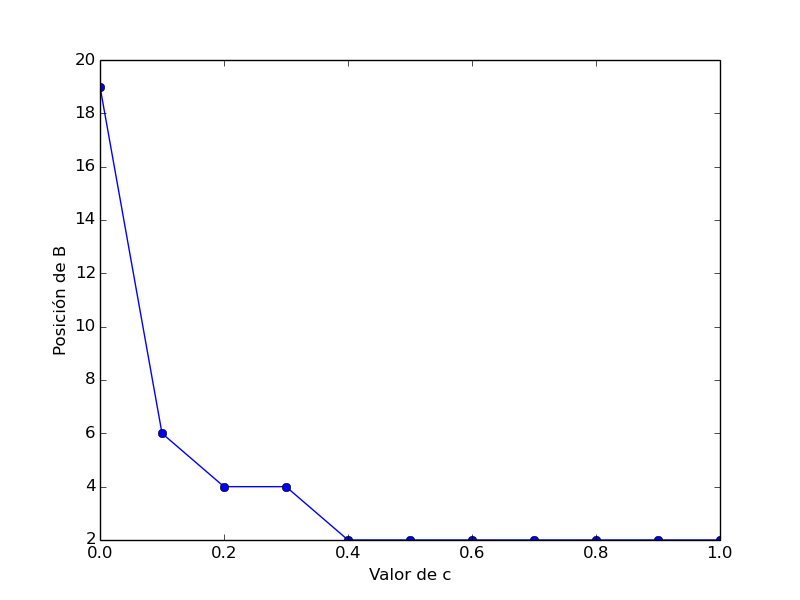
\includegraphics[width=0.5\textwidth]{exp8_posicion_B.png}
    \caption{Posici\'on del equipo B en el ranking en funci\'on del factor
        $\alpha$ ($c=\alpha$)}
    \label{fig:exp8_posB}
\end{wrapfigure}
\noindent
